\subsection{Distribución de Boltzmann}{\label{ap:boltzmann}}

La distribución de Boltzmann se da para todos los sistemas (interactuantes o no) de partículas distinguibles (o clásicas) cuyos potenciales sean independientes de los momentos.
Estos Hamiltoneanos tienen la forma
\[ H(\mathbf{q}_1,..,\mathbf{q}_N,\mathbf{p}_1,..,\mathbf{p}_N) = \sum_{i=1}^N \frac{p_i^2}{2m_i} + U(\mathbf{q}_1,..,\mathbf{q}_N)\]
donde $p_i = |\mathbf{p}_i|$ es el modulo del momento.

Sabiendo que los ensambles son equivalentes en el límite termodinámico, haremos este desarrollo en ensamble canónico por simplicidad.
En este ensamble, la (densidad de) probabilidad de un dado microestado $x=(\mathbf{q}_1,..,\mathbf{q}_N,\mathbf{p}_1,..,\mathbf{p}_N)$ está definida por

\[ P(x) = \frac{e^{-\beta H(\mathbf{q}_1,..,\mathbf{q}_N,\mathbf{p}_1,..,\mathbf{p}_N)}}{\int e^{-\beta H} d^{3N}qd^{3N}p} \]

Aprovechando la forma del Hamiltoneano, la integral del denominador puede factorizarse

\begin{align*}
\int e^{-\beta H} d^{3N}qd^{3N}p &= \int e^{-\beta \left( \sum_i p_i^2/2m_i + U(\mathbf{q}_1,..,\mathbf{q}_N)\right)} d^{3N}qd^{3N}p \\
&= \left(\prod_{i=1}^N\int e^{-\beta\frac{p^2}{2m_i}} d^{3}p\right) \int e^{-\beta U(\mathbf{q}_1,..,\mathbf{q}_N)} d^{3N}q
\end{align*}

Podemos entonces preguntarnos cual es la probabilidad de que una dada partícula $i$ tenga momento $\mathbf{p}_i$.
Esta probabilidad $f_i(\mathbf{p}_i)$ se obtiene integrando sobre todos los posibles estados de las demás partículas y sobre la posición $\mathbf{q}_i$ de la partícula $i$.
Analogamente a la cuenta anterior, vemos que esto arroja

\[ f_i(\mathbf{p}_i) = e^{-\beta\frac{p_i^2}{2m}}\frac{\left(\prod_{j=1, j\neq i}^N\int e^{-\beta\frac{p^2}{2m_j}} d^{3}p\right) \int e^{-\beta U(\mathbf{q}_1,..,\mathbf{q}_N)} d^{3N}q}
{\left(\prod_{j=1}^N\int e^{-\beta\frac{p^2}{2m_j}} d^{3}p\right) \int e^{-\beta U(\mathbf{q}_1,..,\mathbf{q}_N)} d^{3N}q}
= \frac{e^{-\beta\frac{p_i^2}{2m_i}}}{\int e^{-\beta\frac{p^2}{2m_i}} d^3p} \]

Efectuando la integral del denominador, obtenemos finalmente la probabilidad de un dado impulso $\mathbf{p}_i$.
\begin{equation}
f_i(\mathbf{p}_i) = \left(\frac{\beta}{2\pi m_i} \right)^{3/2} e^{-\beta\frac{p_i^2}{2m_i}}
\end{equation}
conocida como distribución de Maxwell-Boltzmann.

Dado que esta probabilidad es isótropa, resultaría natural plantearla en función del módulo del impulso para volverla una distribución de una única variable.
Para esto, debemos integrar en todas las posibles direcciones del vector $\mathbf{p}_i$ además de introducir un jacobiano.
Podemos obtener la nueva distribución aprovechando la normalización y realizando el cambio de variables a esféricas
\[1 = \int f_i(\mathbf{p}_i) d^3p = \int_0^\infty\int_0^{4\pi}\left(\frac{\beta}{2\pi m_i} \right)^{3/2} e^{-\beta\frac{p_i^2}{2m_i}} p^2d\Omega dp 
= \int_0^\infty 4\pi\left(\frac{\beta}{2\pi m_i} \right)^{3/2} p_i^2 e^{-\beta\frac{p_i^2}{2m_i}} dp_i\]
por lo que la probabilidad de que la $i$-esima partícula tenga un momento con módulo $p$ es
\[ f_i(p) = 4\pi\left(\frac{\beta}{2\pi m_i} \right)^{3/2} p^2 e^{-\beta\frac{p^2}{2m_i}} \]

Sin embargo, si todas las partículas son diferentes (por ejemplo, tienen masas $m_i$ diferentes) esta distribución tiene poco valor estadístico, pues no nos otorga información
del sistema en su totalidad. 
Sin embargo, analizar la probabilidad de que la partícula tenga una dada energía cinética $\varepsilon = p^2/2m_i$ permitirá independizarnos de la masa.
Analogamente a lo anterior, planteamos normalización y utilizamos el cambio de variables $2m_i\varepsilon = p^2$ con $d\varepsilon = pdp/m = \sqrt{2m\varepsilon}dp/m$

\[ 1 = \int_0^\infty f_i(p) dp = \int_0^\infty 4\pi\left(\frac{\beta}{2\pi m_i} \right)^{3/2} e^{-\beta\varepsilon} 2m_i\varepsilon\frac{m_i}{\sqrt{2m_i\varepsilon}} d\varepsilon
= \int_0^\infty 2\pi\left(\frac{\beta}{2\pi m_i} \right)^{3/2} e^{-\beta\varepsilon} (2m_i)^{3/2}\sqrt{\varepsilon} d\varepsilon \]

Por lo tanto, la probabilidad de que la $i$-esima partícula tenga una dada energía cinética $\varepsilon$ es identicamente igual para todas las partículas
\begin{equation}
 f(\varepsilon) = \sqrt{\frac{4\beta^3\varepsilon}{\pi}}e^{-\beta\varepsilon}
\end{equation}
y por lo tanto nos permite obtener una propiedad global del sistema. 
Si cada partícula tiene probabilidad $f(\varepsilon)d\varepsilon$ de tener energía cinética $\varepsilon$, entonces la cantidad de partículas con esa energía cinética es $Nf(\varepsilon)d\varepsilon$.
Esta es la distribución de energía cinética del sistema.



\subsection{Cálculo de las funciones de Fermi}

En esta sección, hablaremos del método utilizado para computar las $f_\nu(z)$ con especial interés en el caso $\nu=3/2$ que aparece al buscar $\mu(N,V,T)$
y, en menor medida, el caso $\nu=5/2$ asociado a la presión.

Como dijimos, las funciones de Fermi están definidas según su forma integral, pero pueden expresarse como una serie alternada 
\begin{equation}{\label{eq:fermi_func_serie}}
 f_\nu(z) \equiv \frac{1}{\Gamma(\nu)}\int_0^\infty \frac{x^{\nu-1}}{z^{-1}e^x+1} dx = \sum_{l\geq 1} (-1)^{l+1}\frac{z^l}{l^\nu}
\end{equation}
cuya convergencia resulta lenta para $z$ de orden 1 o mayor.
Sin embargo, para toda $f_\nu(z)$ existirá algún $z_\nu < 1$ que nos asegure una convergencia veloz de las sumas parciales
\[ f_\nu(z) \approx \sum_{l=1}^{m} (-1)^{l+1}\frac{z^l}{l^\nu}\]
para $z\leq z_\nu < 1$.
Esto se debe a que podemos acortar burdamente el error por
\[ \left|f_\nu(z) - \sum_{l=1}^{m}(-1)^{l+1}\frac{z^l}{l^\nu}\right| \leq \sum_{l=m+1}^\infty z^l = z^{m+1}\sum_{l=0}^\infty z^l = z^{m+1} \frac{1}{1-z} \]
donde usamos $z\leq z_\nu < 1$ para resolver la suma geométrica.

Es de esta cota de donde obtendremos el $z_\nu$ que nos asegure un error relativo tolerable.
Por ejemplo, para $m=20$ y $\nu = 3/2$, podemos aproximar $f_\nu(z)$ para $z\leq z_\nu = 0.65$ con sumas parciales cuyo error relativo está acotado por
\[\frac{|f_\nu(z) - \sum_{l=1}^{m}(-1)^{l+1}\frac{z^l}{l^\nu}|}{f_\nu(z)} \leq 10^{-3} = 0.1\%\]

Este error es suficientemente bajo como para afirmar que el método es preciso.
Sin embargo, para $z = 0.75$, el error relativo ya escala a un $2\%$ y para $z=0.8$ al $10\%$, por lo que resulta necesario mejorar el método.
Una forma de lograr esto sería aumentando el $m$ de las sumas parciales, pero esto conlleva el problema inherente de que los sumandos son estrictamente crecientes en módulo para $z\geq 1$.
Eventualmente, estos valores pueden ser suficientemente grandes como para incurrir en \texttt{overflows} o cancelaciones catastróficas.

\subsubsection{Algoritmo de Wynn}

Dado que la expresión de las $f_\nu(z)$ como serie de potencias resulta problemática para $z\geq 1$, podemos recurrir a otras formas.
Una de estas es la aproximación de Padé por una función racional (cociente de polinomios)
\[ [L/M]_{f_\nu}(z) \equiv \frac{P_L(z)}{Q_M(z)} \approx f_\nu(z) \]
donde $P_L(z)$ y $Q_M(z)$ son polinomios de grado $L$ y $M$, respectivamente.
Estos polinomios no nos interesan dado que utilizaremos el \textit{algoritmo $\epsilon$ de Wynn} para obtener las aproximaciones diagonales $[p/p]_{f_\nu}(z) = \epsilon(0, 2p)$ 
donde $\epsilon(n,m)$ está definido recursivamente según
\begin{align*}
 &\epsilon(n, -1) = 0 \\
 &\epsilon(n, 0) = \sum_{l=0}^{n} c_lz^l \\
 &\epsilon(n, m+1) = \epsilon(n+1,m-1) + \frac{1}{\epsilon(n+1,m) - \epsilon(n,m)}
\end{align*}
que, para el caso de las $f_\nu(z)$, son $c_0 = 0$ y $c_l=(-1)^{l+1}/l^\nu$ para $l\geq1$.

Para facilitar la visualización, suelen organizarse los $\epsilon$ en una tabla de doble entrada $n$ y $m$ como se muestra en la \textbf{Figura \ref{fig:wynn_esquema}}.
Allí puede verse claramente que $\epsilon$ deben conocerse para computar $\epsilon(n,m)$.
En particular, en la \textbf{Figura \ref{fig:wynn_ejemplo}} puede verse que (dado que $\epsilon(n,-1)=0$) para computar la aproximación $[p/p]$ basta con computar los $\epsilon(n,m)$ con $0\leq n\leq 2p-m$ y $m\leq 2p$.
Esto corresponde a la mitad superior de la antidiagonal, por lo que la cantidad de cómputos es $(2p)^2/2$.

\begin{figure}[H]
	\centering
	\subfigure[Recurrencia entre elementos]{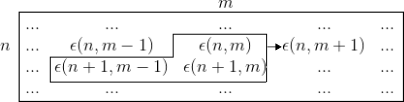
\includegraphics[width=0.26\columnwidth]{apendice/esquema_wynn.png}{\label{fig:wynn_esquema}}}
	\hspace{0.05\columnwidth}
	\subfigure[Ejemplo del cómputo para el caso $p=1$]{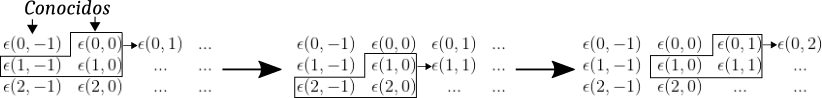
\includegraphics[clip, width=0.68\columnwidth]{apendice/ejemplo_wynn.png}{\label{fig:wynn_ejemplo}}}
	\caption{Arreglo de los coeficientes $\epsilon$ en una tabla para facilitar su cómputo}
	\label{fig:wynn}
\end{figure}

Para una serie de Padé $[p/p]$, el error es $O(z^{2p})$, por lo que tomando $p=10$ podemos obtener un orden similar al de la serie truncada.
Por lo tanto, resultaría razonable utilizar el algoritmo de Wynn para $z\geq z_\nu$, donde (en el caso $\nu=3/2$) empalma con el método de serie truncada con un error 
relativo de $\sim10^{-6}$ más que aceptable. 

Aunque, en general, las $f_\nu(z)$ no poseen una expresión analítica contra la que podamos comparar la eficacia del algoritmo, el caso particular $\nu=1$ si tiene 
expresión analítica: $f_1(z) = \log(z+1)$.
A modo de ejemplo, en la \textbf{Figura \ref{fig:ej_wynn_log}} las aproximaciones a $f_1(z) = \log(z+1)$ mediante el algoritmo de Wynn y sus errores relativos.
Usamos como valor ``exacto'' el arrojado por la función \texttt{log} del paquete \texttt{numpy} de \texttt{Python}.
Puede verse que en el rango $0\leq z\leq 20$, la aproximación con $2p=20$ resulta indistinguible del exacto.

\begin{figure}[H]
	\centering
	\subfigure[Valor absoluto]{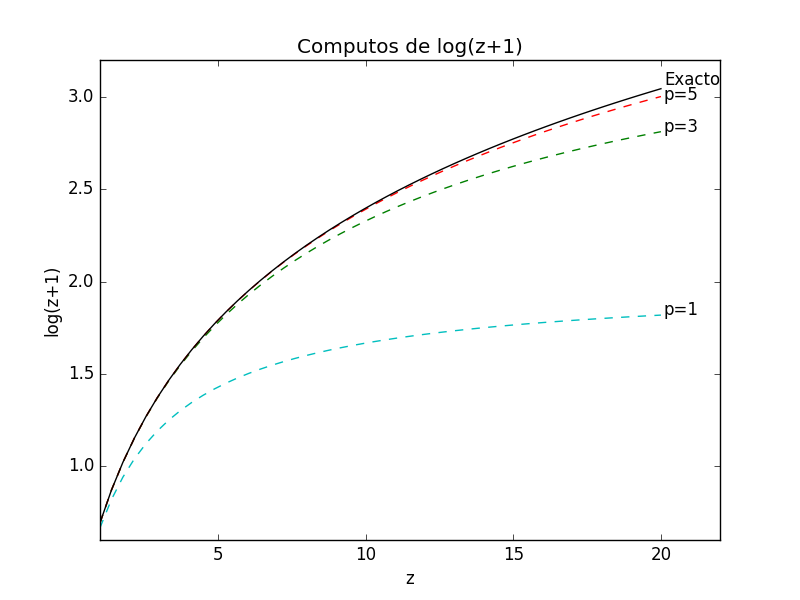
\includegraphics[width=0.4\columnwidth]{apendice/ejemplo_wynn_log.png}}
	\hspace{0.05\columnwidth}
	\subfigure[Error relativo]{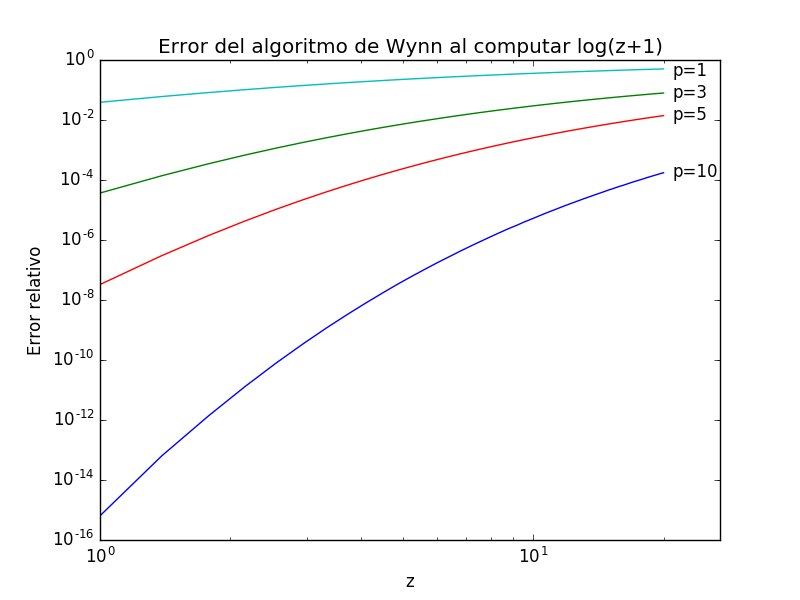
\includegraphics[width=0.4\columnwidth]{apendice/ejemplo_wynn_log_error.png}}
	\caption{Aproximaciones del método de Wynn a la función $f_1(z) = \log(z+1)$, calculada usando el paquete \texttt{numpy} de \texttt{Python}. 
	Podemos ver que rapidamente converge a la función para $p=10$, que resulta indistinguible de la exacta.}
	\label{fig:ej_wynn_log}
\end{figure}

Sin embargo, uno podría preguntarse que nos impide utilizar el algoritmo de Wynn en todo el rango de $z$.
Para $z$ pequeño, dado que las sumas parciales de $\epsilon(n,0)$ convergen rapidamente, la resta que aparece en el demonimador de la definición recursiva de 
$\epsilon(n, m+1)$ tiende a ser menor al número de máquina, transformándolo en una división por $0$.

Para $z$ suficientemente grande, las sumas parciales de $\epsilon(n,0)$ resultan dominadas por el término $z^n$, con $0\leq n\leq 2p$ y $p\sim 10$. 
Por lo tanto, los $\epsilon(n,0)$ se vuelven muy grandes y problemáticos para trabajar para $z\geq 100$. 
Para el caso $\nu=3/2$, observamos las primeras inestabilidades para $z\approx 30$.


\subsubsection{Aproximación de Sommerfeld y forma final}

Para $z$ grande, necesitamos otra forma de computar la $f_\nu(z)$.
Surge la pregunta entonces: ¿existe un $z_m$ suficientemente grande para el cual nos baste conocer $f_\nu(z)$ para $z\leq z_m$?
Esta pregunta surge de recordar el objetivo de partida: encontrar el $z$ que cumple $f_\nu(z)=\frac{N\lambda^3}{gV}\equiv \alpha$.
A priori, $\alpha$ no está acotado superiormente, por lo que necesitamos conocer los $z$ para los cuales $f_\nu(z)\to\infty$.
En particular, estamos interesados en que tanto debemos aumentar $z$ para que $f_\nu(z)$ aumente una dada cantidad.

Para esto, utilizamos el conocido lema de Sommerfeld que nos permite aproximar 
\begin{equation}{\label{eq:sommerfeld}}
 \int_0^\infty \frac{\Phi(x)}{e^{x-\eta}+1}dx = \int_0^\eta \Phi(x) dx + \frac{\pi^2}{6}\left( \frac{d\Phi}{dx} \right)\Bigg|_{x=\eta} + 
 \frac{7\pi^4}{360}\left( \frac{d^3\Phi}{dx^3} \right)\Bigg|_{x=\eta} + ...
\end{equation}

Para el caso de $f_\nu(z)$, podemos usar este lema con $\Phi(x) = x^{\nu-1}/\Gamma(\nu)$ y $z = e^{\eta}$ (o $\eta = \log z$), obteniendo
\begin{equation}{\label{eq:dirac_sommerfeld}}
f_\nu(z) = \frac{1}{\Gamma(\nu)}\left[ \frac{(\log z)^\nu}{\nu} + \frac{\pi^2}{6}(\nu - 1)(\log z)^{\nu-2} + \frac{7\pi^4}{360}(\nu - 1)(\nu - 2)(\nu - 3)(\log z)^{\nu - 4} 
+ O((\log z)^{\nu-6})  \right]
\end{equation}
 
Esto nos dice que para $z$ suficientemente grande, las $f_\nu(z)$ se comportan como potencias del logaritmo de $z$.
Por lo tanto, el crecimiento de $f_\nu(z)$ es considerablemente lento y obtener valores grandes de $f_\nu(z)$ exige valores muchisimo mayores de $z$.
Por ejemplo, utilizar la aproximación de Sommerfeld para resolver $f_{3/2}(z) = 30$ arroja un $z\approx 10^5$. 

Para los valores de $z\geq 20$, utilizamos la aproximación \eqref{eq:dirac_sommerfeld} que empalma en $z=20$ con el algoritmo de Wynn con un error relativo de 
$\sim10^{-3}$ aceptable (para $\nu=3/2$). 

La ventaja de esto es que para $z\geq 20$ tenemos un método explícito y veloz para evaluar $f_{3/2}(z)$, por lo que podemos utilizar algún método para hallar la 
raíz de $g(z) = 0 = f_{3/2}(z) - N\lambda^3/gV$ (en nuestro caso, bisecciones).
Por otro lado, para $0\leq z\leq 20$ construimos una Look-Up Table de $\sim 2500$ puntos, interpolando para obtener los valores de $f_\nu(z)$.
En resumen

\[  \left(\nu = \frac{3}{2}\right) \qquad
 \left\{\begin{matrix}
  0 \leq z \leq 20 & \text{Look-Up Table: } \left\{\begin{matrix}
		    0 \leq z \leq 0.65 & \text{Sumas parciales: } f_{3/2}(z) = \sum_{l=1}^{20} (-1)^{l+1} z^l/l^\nu \\
		    0.65 \leq z \leq 20 & \text{Wynn: } \quad f_{3/2}(z) = \epsilon(0,20) 
		    \end{matrix}\right. \\
 z\geq 20 & \text{Sommerfeld: } \qquad \qquad f_{3/2}(z) = \frac{4(\log z)^{3/2}}{3\pi^{1/2}}\left[ 1 + \frac{\pi^2}{8}(\log z)^{-2} - \frac{7\pi^4}{384}(\log z)^{-4}  \right]
 \end{matrix} \right.
\]

Para calcular las $f_{5/2}(z)$ asociadas a la presión, debimos aumentar el $z_\nu$ hasta $0.75$ manteniendo el límite inferior de Sommerfeld.
Esta aproximación de la $f_{5/2}(z)$ tiene una calidad similar a la de $f_{3/2}(z)$, como se ve en la \textbf{Figura \ref{fig:f32_f52}}.

\begin{figure}[H]
	\centering
	\subfigure[Función $f_{3/2}(z)$ utilizada para obtener $\mu(N,V,T)$]{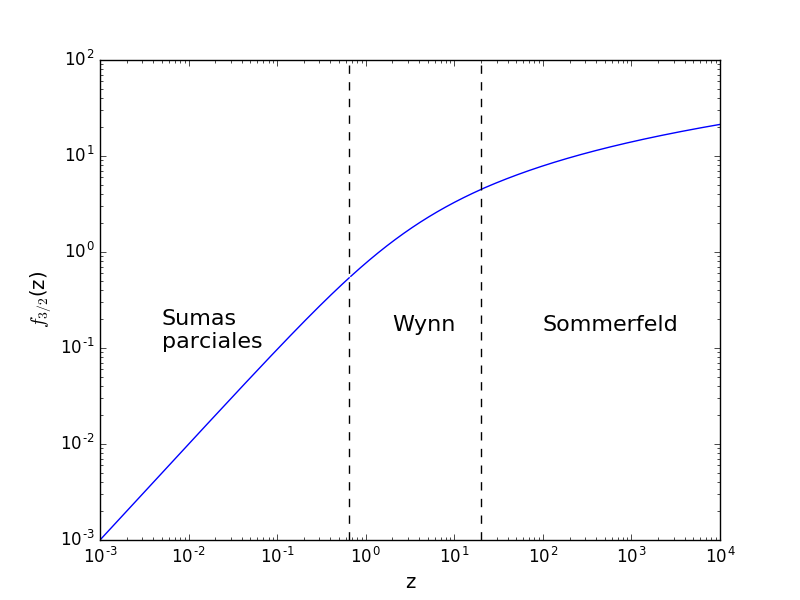
\includegraphics[width=0.4\columnwidth]{apendice/F32.png}}
	\hspace{0.05\columnwidth}
	\subfigure[Función $f_{5/2}(z)$ asociada a la presión del sistema]{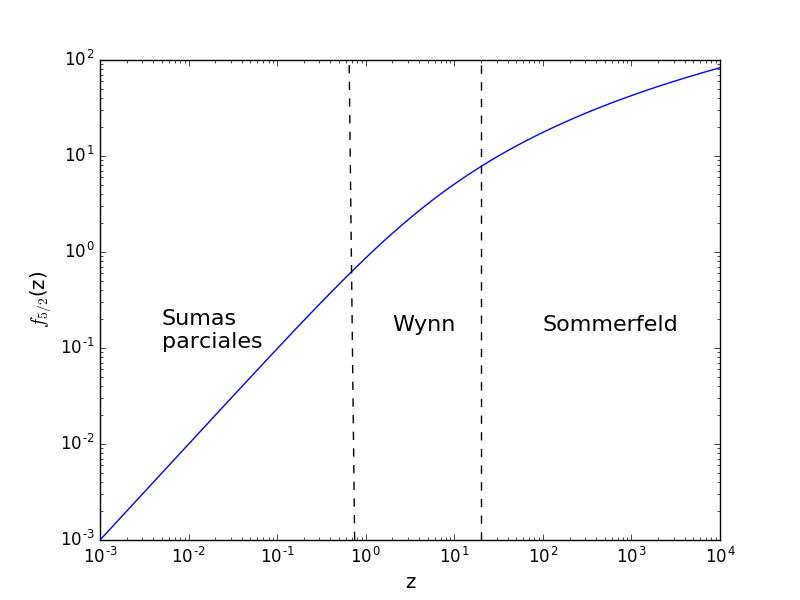
\includegraphics[width=0.4\columnwidth]{apendice/F52.png}}
	\caption{Forma final de las $f_\nu(z)$ utilizando la separación en 3 métodos: sumas parciales, Wynn y Sommerfeld. Puede verse que empalman correctamente.}
	\label{fig:f32_f52}
\end{figure}


\subsection{Integradores no simplécticos: Euler y Runge-Kutta}{\label{sec:no_simp}}

En este apéndice, demostraremos que los métodos de Euler y un Runge-Kutta de orden 2 explícitos no son simplécticos. 
Comenzaremos con el método de Euler de esquema
\[ y_{n+1} = y_n + h J^{-1} \nabla H(y_n) \]
cuya derivada respecto de $y_n$ resulta inmediatamente
\[ \dpart{y_{n+1}}{y_n} = 1 + hJ^{-1}\nabla^2H (y_n)\]
\begin{align*}
 \left( \dpart{y_{n+1}}{y_n} \right)^T J \left( \dpart{y_{n+1}}{y_n} \right) &= \left(1 + h\nabla^2 H(y_n)(J^{-1})^T\right) J \left(1 + hJ^{-1}\nabla^2 H(y_n)\right) \\
 &= \left(1 - h\nabla^2 H(y_n)J^{-1}\right) J \left(1 + hJ^{-1}\nabla^2 H(y_n)\right) \\
 &= J - \cancel{h\nabla^2 H(y_n)} + \cancel{h\nabla^2 H(y_n)} - h^2\nabla^2 H(y_n)J^{-1}\nabla^2 H(y_n) \neq J
\end{align*}

Por otro lado, el método Runge-Kutta de orden 2 con esquema
\[ y_{n+1} = y_n + h J^{-1} \nabla H\left(y_n + \frac{h}{2} J^{-1} \nabla H(y_n) \right) \equiv y_n + h J^{-1} \nabla H\left(y_{n+1/2} \right) \]
tiene una derivada respecto de $y_n$ más complicada
\[ \dpart{y_{n+1}}{y_n} =  1 - h\left[ 1 - \frac{h}{2} \nabla^2 H(y_n)J^{-1} \right]\nabla^2H\left(y_n + \frac{h}{2} J^{-1} \nabla H(y_n)J^{-1} \right) \equiv 1 - h\left[ 1 - \frac{h}{2} \nabla^2 H(y_n)J^{-1} \right]\nabla^2H\left(y_{n+1/2} \right) \]
\begin{align*}
 \left( \dpart{y_{n+1}}{y_n} \right)^T &J \left( \dpart{y_{n+1}}{y_n} \right) \\
 &= \left( 1 - h\left[ 1 - \frac{h}{2} \nabla^2 H(y_n)J^{-1} \right]\nabla^2H\left(y_{n+1/2} \right)J^{-1} \right) J \left(1 + hJ^{-1}\nabla^2H\left(y_{n+1/2} \right)\left[ 1 + \frac{h}{2} J^{-1} \nabla^2 H(y_n) \right] \right)\\
 &= J + \frac{h^2}{2} \nabla^2 H(y_n)\nabla^2H(y_{n+1/2}) + \frac{h^2}{2} \nabla^2H(y_{n+1/2})\nabla^2 H(y_n) -\\
 &\qquad - h^2\left[ 1 - \frac{h}{2} \nabla^2 H(y_n)J^{-1} \right]\nabla^2H(y_{n+1/2}) J^{-1}\nabla^2H(y_{n+1/2})\left[ 1 + \frac{h}{2} J^{-1} \nabla^2 H(y_n) \right] \\
 &= J + \frac{h^2}{2} \left[ \nabla^2 H(y_n)\nabla^2H(y_{n+1/2}) +  \nabla^2H(y_{n+1/2})\nabla^2 H(y_n) - 2\nabla^2H\left(y_{n+1/2} \right) J^{-1}\nabla^2H(y_{n+1/2}) \right] \\
 &\quad + \frac{h^3}{2} \left[ \nabla^2H(y_{n+1/2}) J^{-1}\nabla^2H(y_{n+1/2})J^{-1} \nabla^2 H(y_n) - \nabla^2 H(y_n)J^{-1}\nabla^2H(y_{n+1/2}) J^{-1}\nabla^2H(y_{n+1/2})\right] \\
 &\quad + \frac{h^4}{4} \nabla^2 H(y_n)J^{-1}\nabla^2H(y_{n+1/2}) J^{-1}\nabla^2H(y_{n+1/2})J^{-1}\nabla^2 H(y_n)
\end{align*}

Para anular los ordenes cuadrático y cúbico, se requiere basicamente $\nabla^2H(y_n) = \nabla^2H(y_{n+1/2})$, pero el término cuártico en $h$ es no nulo.
Por lo tanto, este método RK2 no es simpléctico.

\subsubsection{Implementación de interacción de Pauli}

